‘Home’ fanen for en administrerende bruger er forskellig på nogle punkter, men ellers er layoutet meget af det samme. Nyhedsfeedet viser aktiviteter, såsom hvilket barn der påtog sig en eller anden pligt, eller at der er blevet anmodet om at en pligt er færdig, og er klar til at blive evalueret af administrator brugeren. På dette vindue bliver der også vist en notifikation af hvor mange anmodninger der afventer evaluering. Derudover er der også knapper, som fører brugeren over i et nyt vindue, hvor brugeren kan lave nye pligter eller almindelig bruger profiler, som vil blive lagt op på databasen. Se figur \ref{ForalderUI} for at se dette og de andre faner.

Fanen for ‘Pligter’ viser i dette eksempel en samlet liste for alle pligter, hvor ledige pligter bliver vist nederst på listen, påtaget pligter i midten, og pligter som afventer evaluering af en administrator bruger i toppen. I denne faner er der igen en knap til at lave en pligt. Derudover er der en  redigeringsknap, som skulle gøre det muligt at ændre på en markeret pligt i listen. Der er også knapper til acceptere og afvise en af pligterne som er anmodet til at være færdige, hvorefter den markerede pligt vil blive opløst i systemet, hvis den blev accepteret, og en transaktion vil blive sendt til den pågældende bruger. Ellers vil den blive sat tilbage til at være en påtaget pligt. 

Statistik fanen vil her, til forskel fra den almindelige bruger, vise statistik for alle de almindelige brugere i systemet, hvor den almindelige bruger kun ville kunne se statistik for sig selv. Den administrerende bruger har dog ikke nogen liste over saldo ændringer, da denne slags bruger ikke har en konto i dette system. 

‘Børn’ fanen ville ligesom ‘Pligter’ fanen vise en liste over de almindelige brugere i systemet, og vise diverse informationer angående dem. For eksempel hvad for noget pligter en bruger har påtaget, samt statussen på disse pligter, og saldo. Derudover ville fanen også give muligheder til at lave en ny almindelig bruger til systemet, samt muligheden for at hæve på en af brugernes konti, efter anmodning fra brugeren.

\begin{figure}[H]
\centering
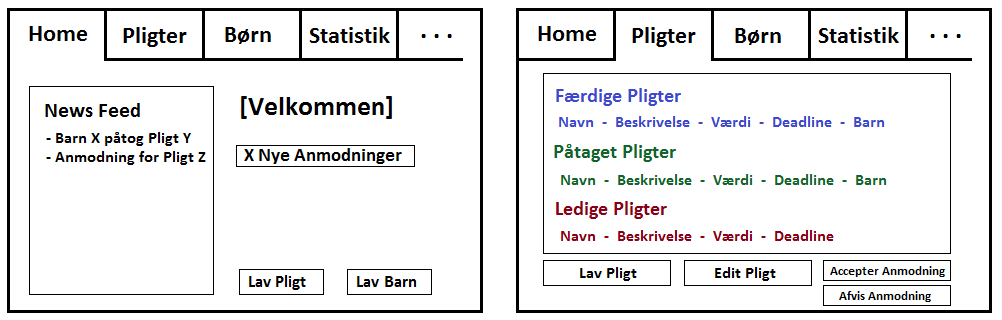
\includegraphics[width=0.9\textwidth]{Billeder/ForalderUI.png}
\caption{Brugergrænseflade illustration for administrerende brugere.}
\label{ForalderUI}
\end{figure}
